\documentclass[nocover]{pset}
\usepackage{tikz-cd}
\usepackage{fancyhdr}
\usepackage{changepage}
\usepackage{mdframed}
\newmdenv[
  innerleftmargin = 1em,
  innertopmargin = 0pt,
  innerbottommargin = 0pt,
  innerrightmargin = 0pt,
  rightmargin = 0pt,
  leftmargin = 1em,
  linewidth = 2pt,
  topline = false,
  rightline = false,
  bottomline = false
  ]{leftbar}
\newcommand{\dom}{\mrm{dom}}
\newcommand{\cod}{\mrm{cod}}
\newcommand{\ob}{\mrm{ob}}
\newcommand{\homm}{\mrm{hom}}
\newcommand{\id}{\mrm{\id}}

\begin{document}
\pagestyle{fancy}
\fancyhf{}
\lhead{Forest Kobayashi}
\chead{Basic Category Theory}
\rhead{Math 196 -- Fall, 2018}
\rfoot{\thepage\ of \pageref{LastPage}}
\setlength{\headheight}{15.2pt}
\setlength{\headsep}{10pt}

\lfoot{Thursday, September 13th 2018}

\begin{center}
  {\scshape \LARGE Basic Category Theory}

  {\scshape (Pseudo)-lecture 1}
\end{center}
\hrulefill

\section*{Introduction}
Often in mathematics, we are interested in considering collections of
objects with structure, and how that structure is modified or
preserved when mapping to some other object. Category theory makes
this a little more formal. First, we begin with some definitions.\\

\subsection*{Meta-objects}
\begin{definition}[Metagraph]
  A \emph{metagraph} consists of any collection (note: does not mean a
  set! See \emph{proper classes}) of \emph{objects} $o_1, o_2,
  \ldots$ (not necessarily countable), and \emph{arrows} $a_1, a_2,
  \ldots$, together two operations that allow us to put the two in
  correspondence:\\
\end{definition}
\begin{definition}[Domain \& Codomain]
  \emph{Domain}, which assigns to each arrow $a_i$ an object $o_j =
  \mrm{dom}(a_i)$, and \emph{Codomain}, which assigns to each arrow
  $a_i$ an object $o_k = \mrm{cod}(a_i)$.
\end{definition}

As is convention, we denote the above with one of the following
diagrams:
\begin{figure}[H]
  \centering
  \begin{minipage}{.33\linewidth}
    \[
      a_i : o_j \to o_k
    \]
  \end{minipage}
  \begin{minipage}{.33\linewidth}
    \begin{tikzcd}
      o_j \arrow[r, "a_i"] & o_k
    \end{tikzcd}
  \end{minipage}
  \caption{Equivalent representations of the above}
\end{figure}
Of course, these diagrams can become quite complicated:
\begin{figure}[H]
  \centering
  \begin{tikzcd}
    o_1
    \arrow[drr, bend left, "a_1"]
    \arrow[ddr, bend right, "a_2"]
    \arrow[dr, "a_3"] & & o_2 \arrow[d, "a_8"]& \\
    & o_3 \arrow[r, "a_4"] \arrow[d, "a_5"] \arrow[ur, "a_9"]
    & o_4 \arrow[d, "a_6"] & \\
    & o_5 \arrow[r, "a_7"] & o_6
  \end{tikzcd}
  \caption{Complicated diagram}
\end{figure}
Using these metagraphs, we can construct a \emph{metacategory}:
\begin{definition}[Metacategory]
  A \emph{metacategory} is a metagraph, with the addition of two more
  operations:

  \emph{Identity}, which maps each object to an ``identity'' arrow:
  \[
    id(o) = 1_o : o \to o;
  \]
  \emph{Composition}, which maps a pair of arrows $a_1, a_2$ (with
  $\mrm{\dom(a_1) = \cod(a_2)}$) to a ``composite'' arrow, $a_1 \circ
  a_2$, such that composition is associative:
  \begin{figure}[H]
    \centering
    \begin{tikzcd}
      \dom(a_2) \arrow[rd, "a_2\circ a_1"] \arrow[r, "a_2"] & \cod(a_2) =
      \dom(a_1) \arrow[d, "a_1"]\\
      & \cod(a_1)
    \end{tikzcd}
  \end{figure}
  and for all arrows $a_1
  : o_1 \to o_2$, $a_2 : o_2 \to o_3$, $\exists$ an identity arrow
  $1_{o_2}$ such that
  \begin{figure}[H]
    \centering
    \begin{minipage}{.49\linewidth}
      \centering
      \begin{tikzcd}
        o_1 \arrow[r, "a_1"] \arrow[dr, "a_1"] & o_2
        \arrow[d, "1_{o_2}"]\\
        & o_2
      \end{tikzcd}
    \end{minipage}
    \begin{minipage}{.49\linewidth}
      \centering
      \begin{tikzcd}
        o_2 \arrow[d, "1_{o_2}"] \arrow[dr, "a_2"]& \\
        o_2 \arrow[r, "a_2"]& o_3
      \end{tikzcd}
    \end{minipage}
    \caption{Identity arrows}
  \end{figure}
  commute.
\end{definition}

\subsection*{Categories, proper}
In order to actually work with the objects we're used to commonly
seeing in mathematics, we'll have to narrow our scope a bit. Notably,
instead of considering a general \emph{collection} of objects, we'll
instead restrict ourselves to just sets. Hence, we can't consider the
category of all categories, and whatnot. We skip the definition of a
directed graph (``diagram scheme''), and jump straight to categories.
Basically, we summarize the metacategory properties, just specifying
that we're using sets now:

\begin{definition}[Category]
  A \emph{category} $C$ consists of
  \begin{enumerate}[label=\arabic*)]
    \item A set $\ob(C)$ of \emph{objects},
    \item A set $\homm(C)$ of \emph{arrows},
    \item A function $\mrm{id} : \ob(C) \to \homm(C)$, by $o \mapsto
      1_o$,
    \item And a function $\circ : \homm(C) \times_{\ob(C)} \homm(C)
      \to \homm(C)$ (with $\times_{\ob(C)}$ giving composable pairs)
      with $(a_1, a_2) \mapsto a_1 \circ a_2$
  \end{enumerate}
\end{definition}

A few terms:
\begin{enumerate}
  \item A category with every arrow identity is called
    \emph{discrete}.
  \item A group is a category with just a single object. Here, the
    object really just represents the ``group itself.'' The arrows are
    morphisms, which we can think of as being ``left multiply by $a$''
    or ``right multiply by $a$.''
\end{enumerate}

\subsection*{Functors}
One key aspect of category theory that will be of particular interest
to us is how we can translate structure from one space to another.
This is the basis for, among other things, the field of representation
theory. Here, we want to not only to put objects in correspondence
with each other, but also preserve the morphism structure on them. In
this sense, a functor is a morphism of categories.

\begin{definition}[Functor]
  Let $C, D$ be categories, and let $c \in \ob(C)$, $f,g \in
  \homm(C)$. Then call $\mc{F} = (\mc{F}_o, \mc{F}_a)$ a functor if
  \[
    \mc{F}_o : \ob(C) \to \ob(D) \qquad \mc{F}_a : \homm(C) \to
    \homm(D)
  \]
  such that the following essential properties are preserved:
  \begin{enumerate}
    \item $\forall (f : c \to c') \in \homm(C)$, $\mc{F}_a(f) :
      \mc{F}_o(c) \to \mc{F}_o(c')$, with
      \[
        \mc{F}_a(1_{c}) = 1_{\mc{F}_o(c)}
      \]
      and
      \[
        \mc{F}_a(g \circ f) = \mc{F}_a(g) \circ \mc{F}_a(f).
      \]
  \end{enumerate}
\end{definition}
before we go on, let's take a moment to really think what's going on
here in terms of our diagrams. Loosely speaking, we're finding ways of
folding our diagrams in on themselves such that we don't put two pairs
of antiparallel arrows together. This is best expressed with a
picture:
\begin{figure}[H]
  \centering
  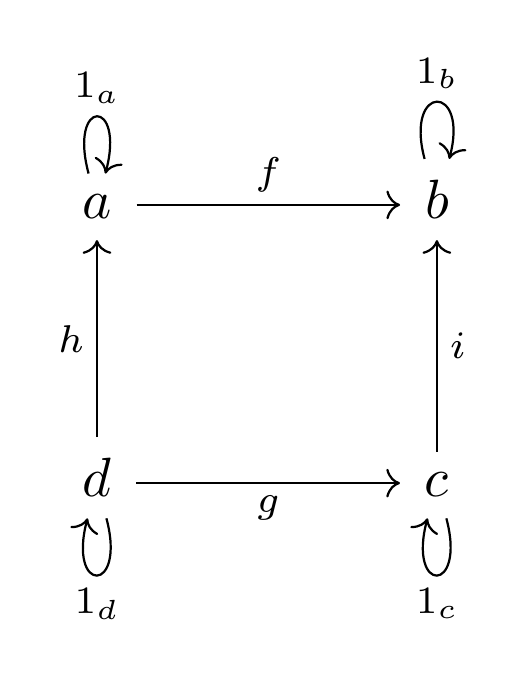
\begin{tikzpicture}
    \node[scale=2] (a) at (0,0) {
      \begin{tikzcd}
        a \arrow[rr, "f"] \arrow[loop above, "1_a"]&  & b
        \arrow[loop above, "1_b"]\\
        &  &  \\
        d \arrow[rr, "g"'] \arrow[uu, "h"] \arrow[loop below,
        "1_d"] &  & c \arrow[uu, "i"'] \arrow[loop below,
        "1_c"]
      \end{tikzcd}
    };
  \end{tikzpicture}
  \caption{Example starting category $C$}
\end{figure}
Suppose we want to map to the following category $D$:
\begin{figure}[H]
  \centering
  \begin{tikzpicture}
    \node[scale=2] (a) at (0,0) {
      \begin{tikzcd}
        &  & c' \arrow[loop above, "1_{c'}"] \\
        & b' \arrow[ru, "g'"] \arrow[loop above, "1_{b'}"] &  \\
        a' \arrow[ru, "f'"] \arrow[loop above, "1_{a'}"]&  &
      \end{tikzcd}
    };
  \end{tikzpicture}
  \caption{Mapped-to category $D$}
\end{figure}
One way we could do so would be to define the following functor:
\begin{align*}
  \mc{F}_o(d) &= a' \\
  \mc{F}_o(a) &= b' \\
  \mc{F}_o(c) &= b' \\
  \mc{F}_o(b) &= c'
\end{align*}
and
\begin{align*}
  \mc{F}_a(1_a) &= 1_{b'} & \mc{F}_a(f) &= g' \\
  \mc{F}_a(1_c) &= 1_{c'} & \mc{F}_a(i) &= g' \\
  \mc{F}_a(1_d) &= 1_{a'} & \mc{F}_a(g) &= f' \\
  \mc{F}_a(1_b) &= 1_{c'} & \mc{F}_a(h) &= f'
\end{align*}
visually, we can interpret this as follows:
\begin{figure}[H]
  \centering
  \begin{tikzpicture}
    \node[scale=.8] (a) at (-7,0) {
      \begin{tikzcd}
        a \arrow[rr, "f"] \arrow[loop above, "1_a"]&  & b
        \arrow[loop above, "1_b"]\\
        &  &  \\
        d \arrow[rr, "g"'] \arrow[uu, "h"] \arrow[loop below,
        "1_d"] &  & c \arrow[uu, "i"'] \arrow[loop below,
        "1_c"]
      \end{tikzcd}
    };

    \node[scale=.8] (b) at (0,0) {
      \begin{tikzcd}
        &  &  & b \arrow[loop above, "1_{b}"] \\
        & a \arrow[rru, "f"] \arrow[loop above, "1_{a}"] &  &  \\
        &  & c \arrow[ruu, "i"'] \arrow[loop below, "1_{c}"] \\
        d \arrow[rru, "g"] \arrow[ruu, "h"] \arrow[loop below,
        "1_{d}"] &  &  &
      \end{tikzcd}
    };

    \draw[dotted, -latex] (-5.5,0) -- (-1.5,0) node[above, midway] {About
      to apply $\mc{F}$};

    \node[scale=.8] (c) at (7,0) {
      \begin{tikzcd}
        &  & c' \arrow[loop above, "1_{c'}"] \\
        & b' \arrow[ru, "g'"] \arrow[loop above, "1_{b'}"] &  \\
        a' \arrow[ru, "f'"] \arrow[loop above, "1_{a'}"]&  &
      \end{tikzcd}
    };

    \draw[-latex] (1.5,0) -- (5.5,0) node[above, midway] {Actually
      applying $\mc{F}$};
  \end{tikzpicture}
  \caption{Demonstration of ``folding''}
\end{figure}
Do in ``class'' --- attempt to prove this is a valid way of thinking
about stuff.

Just as we have ``surjective'' and ``injective'' functions, so too do
we have ``full'' and ``faithful'' functors.\\

\begin{definition}
  A functor $\mc{F} : C \to D$ is called \emph{full} if $\forall c,c'
  \in \ob(C)$, $\forall g : \mc{F}_o(c) \to \mc{F}_o(c')$, $\exists f
  : c \to c' \st g = \mc{F}_a(f)$. Note that this is \emph{not} the
  same thing as being surjective with respect to morphisms and
  objects. In the case of objects, it is quite clear that it need not
  be surjective. With respect to morphisms, this is not quite so.
  However it \emph{does} have to be surjective on
  $\homm(\mc{F}_o(\ob(C)))$. Basically, if we forget about all the
  objects with only the identity morphism defined on them (call this
  resulting category $C'$), then fullness requires that $C'$ map to an
  isomorphic directed sub-graph in $D$ under $\mc{F}$.\\
\end{definition}

\begin{definition}
  A functor $\mc{F} : C \to D$ is called \emph{faithful} if $\forall
  c, c' \in C$, $\forall f_1, f_2 : c \to c'$, then $\mc{F}_a(f_1) =
  \mc{F}_a(f_2) : \mc{F}_o(c) \to \mc{F}_o(c')$ implies $f_1 = f_2$.
  Again, $\mc{F}$ need not be injective on $\ob(D)$, $\homm(D)$. The
  object case is fairly apparent, but with respect to morphisms, it's
  again a little more subtle. Essentially, faithfullness is only
  requiring that if we have two morphims \emph{with the same domain
    and codomain} in $C$, we can't ``squish'' them together in $D$.
  However, morphisms with different domains and codomains can be
  assigned to the same morphism in $D$.
\end{definition}

\begin{definition}
  Subcategories are defined as one might expect a subset of objects
  and arrows such that for each arrow, we have both domain and
  codomain, for each object, we have identity arrow, and for each
  composable pair, we have their composite.
\end{definition}

\section*{Natural Transformations}
As it turns out, it's turtles all the way down. We now want to discuss
morphsims of functors.

\begin{definition}
  Let $C,D$ be categories, and let $\mc{F}, \mc{G} : C \to D$ be
  functors. Then call $\eta$ a natural transformation if
  \begin{enumerate}[label=\arabic*)]
    \item $\forall c \in C$, $\eta$ assigns to $c$ a morphism $\eta_c
      : \mc{F}_o(c) \to \mc{G}_o(c)$, called the \emph{component} of
      $\eta$ at $c$. This $\eta_c$ must satisfy
    \item $\forall f : c \to c'$, we have that $\eta_{c'} \circ
      \mc{F}_a(f) = \mc{G}_a(f) \circ \eta_c$
      \begin{figure}[H]
        \centering
        \begin{tikzcd}
          \mc{F}_o(c) \arrow[rr, "\eta_c"] \arrow[dd, "\mc{F}_a(f)"'] &
          & \mc{G}_o(c) \arrow[dd, "\mc{G}_a(f)"] \\
          &  &  \\
          \mc{F}_o(c') \arrow[rr, "\eta_{c'}"] &  & \mc{G}_o(c')
        \end{tikzcd}
        \caption{Natural transformation}
      \end{figure}
  \end{enumerate}
\end{definition}
Essentially, this ``glues'' diagrams of functors together such that
moving around the ``image'' one the $\mc{F}$ side and then hopping
over to the $\mc{G}$ side leaves you in the same place as first
hopping over to the $\mc{G}$ side and then taking an analogous path
there (draw on board maybe). If $\eta$ is invertible (that is, if
every component of $\eta$ is invertible), then we call $\eta$ a
\emph{natural isomorphism} or \emph{natural equivalence}.

Example: determinants, ring homomorphisms, and matrices. Can either
apply (matrix) ring homomorphism first, then take det, or take det,
then apply ring (matrix entries) homomorphism. Either gets the same
result.

\section*{Monics, Epics, and Zeros.}
Epic indeed. One might be wondering, \emph{how the heck does this
  whole ``groups as categories with one objec'' thing play out? How do
we distinguish between two morphisms, if they have the same domain and
codomain?} All fantastic questions. Let's jump right into it.

In category theory, our primary focus will largely be on
\emph{morphisms}. As MacLane states, this is part of the power of
Category Theory --- instead of thinking about properties in terms of
element-by-element treatments, we can instead think of them in terms
of morphisms that sort of ``take us between states.'' hence, we bring
a slew of definitions.\\

\begin{definition}[Invertible morphisms]
  Let $C$ a category, and $f : c \to c' \in \homm(C)$. Call $f$
  \emph{invertible} if $\exists f^{-1} : c' \to c \in \homm(C) \st
  f\circ f^{-1} = 1_{c'}$, and $f^{-1} \circ f = 1_c$. Then $f^{-1}$
  is unique, and $f, f^{-1}$ are called \emph{isomorphisms}.\\
\end{definition}
\begin{definition}[Isomorphism]
  Call $c, c' \in \ob(C)$ \emph{isomorphic} if there is an isomorphism
  between them.\\
\end{definition}
\begin{definition}[Monic]
  Let $a,c,c' \in \ob(C)$, and let $m \in \homm_C(c', a)$. Call $m$
  \emph{monic} if $\forall f_1, f_2 \in \homm_C(c,c')$, $m \circ f_1 =
  m \circ f_2 \implies f_1 = f_2$. Basically, $m$ never jumbles up
  parallel arrows from $c$ to $c'$, provided you apply it \emph{after}
  the arrows. It is always \emph{left}-cancellable, and sort of
  ``always preserves information in the domain.''\\
\end{definition}
\begin{definition}[Epi]
  Epis are defined similarly, but are \emph{right}-cancellable. In
  some sense, it never loses information in the co-domain.\\
\end{definition}
\begin{definition}[Right \& Left Inverses]
  Right and left inverses are defined in the expected manner. Let $C$
  a category, and $f \in \homm_C(c,c')$. Then $s \in \homm_C(c', c)$
  is called a \emph{right} inverse or \emph{section} of $f$ if $f\circ
  s = 1_{c'}$, and a \emph{left} inverse or \emph{retraction} if
  $s\circ f = 1_c$. \\
\end{definition}
If $f$ has a right inverse, it is epi, if it has a left inverse, it is
monic. However the converse of these statements do not necessarily
hold. Am still slightly confused about that; remember to ask Prof.
Nelson.

Let $g \in \homm_C(c',c)$, $h \in \homm_C(c,c')$. Then if $g\circ h =
1_c$, call $g$ a \emph{split epi}, $h$ a \emph{split monic}, and $f =
h\circ g$, call $f$ idempotent.

\begin{definition}[Terminal]
  Call an object $c$ \emph{terminal} if $\forall c' \in \ob(C)$,
  $\exists ! f : c' \to c$. \\
\end{definition}

\begin{definition}[Initial]
  Call an object $c$ \emph{initial} if $\forall c' \in \ob(C)$,
  $\exists ! f : c \to c'$. \\
\end{definition}

\begin{definition}[Null]
  Call an object $c$ \emph{null} if it is both initial and terminal.
\end{definition}

\end{document}
